\section{Introduction}
% Training of deep neural networks usually requires lots of input data and according labels.
% Especially in the medical imaging domain only a few images and even less labels are available due to annotation costs especially for pixel-wise semantic segmentation tasks \citep{bhalgat2018annotation}.

Deep neural networks dominate the state-of-the-art medical image segmentation \citep{liu2021review,ronneberger2015u,isensee2021nnu}, but their high performance is depending on the availability of large-scale labelled datasets.
Such labelled data is often not available in the target domain and direct transfer learning leads to performance drops due to domain shift \citep{yan2019domain}.
% While deep neural networks often achieve outstanding results on semantic segmentation tasks within a dataset domain, results can drop significantly when predicting on domain-shifted input data \citep{yan2019domain}.
To overcome these issues transferring existing annotations from a labeled source to the target domain is desirable.
% Multi-atlas segmentation aims at transferring multiple available sample annotations to target images via image registration. After registration multiple “optimal” labels for a sample exist, which require a decision for the “best” candidate or consensus \citep{artaechevarria2009combination}. A consensus in turn can then be used to train neural networks for the new domain.
Mutli-atlas segmentation is a popular method, which accomplishes such a label transfer in two steps:
First, multiple sample annotations are transferred to target images via image registration \citep{marstal2016simpleelastix,heinrich2012globally,siebert2021fast} resulting in multiple ``optimal'' labels \citep{artaechevarria2009combination}.
Secondly label fusion can be applied to build the label consensus.
% Although many methods for finding a consensus label have been developed they might not necessarily provide the best possible input for a consecutive neural network training due to non-optimal registration and fusion.
Although many methods for finding a consensus label have been developed \citep{artaechevarria2009combination,heckemann2006automatic,rohlfing2004performance,warfield2004simultaneous,wang2013multi}, the resulting fused labels are still not perfect and exhibit label noise, which complicates the training of neural networks and degrades performance.
% 4. In this work, we aim to mitigate this problem of label noise and propose to learn a sem segm model along with ...

% \paragraph{\textbf{Motivation}}
% \label{sec:motivation}
% The pixel-wise classification i.e. segmentation performance of organs and structures of interest in medical imaging has been improved significantly over the past years \citep{liu2021review,ronneberger2015u,isensee2021nnu}.
% Although segmentation within an imaging domain like CT or MRI can work well, problems arise when no target label data is available and the segmentation task on target data contains a domain shift \citep{yan2019domain}.
% As stated before, problems arise when no target label data is available and the segmentation task on target data contains a domain shift.
% As stated before, one way to overcome a domain shift in data is propagating labels from the source domain to the target domain via image registration \citep{marstal2016simpleelastix,heinrich2012globally,siebert2021fast}. A propagated label could be used directly as a solution for the target label, but in general image registration is a challenging task and a “perfect” registration is hard to obtain \citep{xu2016evaluation}.

\paragraph{\textbf{Related work}}
\label{sec:related}
In the past, various label fusion methods have been proposed,
% which take several registered candidates as input and output a common consesus label via a non-trivial weighted voting task
which use weighted voting on registered label candidates to output a common consensus label
\citep{artaechevarria2009combination,heckemann2006automatic,rohlfing2004performance,warfield2004simultaneous}.
More elaborate fusion methods also use image intensities \citep{wang2013multi}, however when predicting across domains source and target intensities can differ substantially complicating intensity-based fusion and would therefore require handling of the intensity gap i.e. with image-to-image translation techniques \citep{zhu2017unpaired}.
When using the resulting consensus labels from non-optimal registration and fusion for subsequent CNN training, noisy data is introduced to the network \citep{karimi2020deep}.
Network training can then be improved with techniques of curriculum learning to estimate label noise (i.e. difficulty) and guide the optimization process accordingly \citep{saxena2019data,castells2020superloss} but the techniques have not been used in the context of noise introduced through registered pixel-wise labels \citep{bengio2009curriculum,saxena2019data,castells2020superloss,jiang2018mentornet,zhang2020distilling} or employ more specialized and complex pipelines \citep{ding2019votenet,ding2020votenet+,liu2021style}.
Other deep learning-based techniques to address ambiguous labels are probabilistic networks \citep{kohl2018probabilistic}.

% Alex

% The primary methodological focus of our work lies on training a medical segmentation model in the presence of label noise. Previous approaches to this problem can be grouped into ?? categories (see  [Deep learning with noisy labels: exploring techniques and remedies in medical image analysis] for a comprehensive survey).

% 1) [Minimal annotation training for segmentation of microscopy images] and [Ct organ segmentation using gpu data augmentation, unsupervised labels and iou loss] introduced robust loss function to mitigate negative effects of label noise.

% 2) In a different approach, [Robust learning at noisy labeled medical images: Applied to skin lesion classification] proposed a data re-weighting scheme, which removes samples with high loss values from each batch.

% 3) [A two-stream mutual attention network for semi-supervised biomedical segmentation with noisy labels] proposed to address label noise by a specific training procedure, involving two networks, which are only updated if the networks disagree. That way, the authors intend to identify hard examples with correct labels.

% 4) Specific model architecture: probabilisic U-Net, VoteNet, VoteNet+

% Contrary to these methods, we propose to automatically learn the quality of noisy labels through data parameters, which are learnt jointly with network weights. The concept of data parameters was introduced by Saxena et al. \citep{Saxena} and can be classified as a method from curriculum learning. Further works in this area include \citep{bengio2009curriculum,Castells.2020,jiang2018mentornet,Zhang.1022019} but the techniques have not been used in the context of noise introduced through registered pixel-wise-labels.

% 3. Even though not the primary methodological focus, our work is also related to label propagation and fusion throuh  registration.  --> hier kannst du dann noch den Anfang vom related Work Teil einbauen --> wobei du das denke ich auch noch etwas kürzer fassen kannst.

\paragraph{\textbf{Contributions}}
\label{sec:contributions}
We propose to use data parameters \citep{saxena2019data} to weight noisy atlas samples as a simple but effective extension of semantic segmentation models. During training the data parameters (scalar values assigned to each instance of a registered label) can estimate the label trustworthiness globally across all multi-atlas candidates of all images.
We extend the original formulation of data parameters by additional \emph{risk regularization} and \emph{fixed weighting} terms to adapt to the specific characteristics of the segmentation task and show that our adaptation improves network training performance for 2D and 3D tasks in the single-atlas scenario.
Furthermore, we apply our method to the multi-atlas 3D image scenario where the network scores do not improve but yield equal performance in comparison to normal cross-entropy loss training when using {out-of-line backpropagation}.
Nonetheless, we still can achieve an improvement by deriving an optimized consensus label from the extracted weights and applying a straightforward weighted-sum on the registered atlases.

% \newpage
\section{Methods}
\label{sec:method_deepstaple}
    In this section, we will describe our data parameter adaption\footnote{Our code is openly available on GitHub: \url{https://github.com/multimodallearning/deep_staple}} and introduce our proposed extensions when using it in semantic segmentation tasks, namely a special regularization and a fixed weighting scheme. Furthermore, a multi-atlas specific extension will be described, which improves training stability.
    \paragraph{\textbf{Data parameters}}
        \label{sec:data_parameters}
        Saxena et al. \citep{saxena2019data} formulate their data parameter and curriculum learning approach as a modification altering the logits input of the loss function.
        By a learnable logits-weighting improvements could be shown in different scenarios when either noisy training samples and/or classes were weighted during training.
        Our implementation and experiments focus on per-sample parameters \(\mathbf{DP_{S}}\) of a dataset \(S=\left\{\left(\mathbf{x_s}, \mathbf{y_s}\right)\right\}_{s=1}^{n}\) with images \(x_s\) and labels \(y_s\) containing \(n\) training samples.
        % determining noisy multi-atlas samples. Experiments were conducted on binary semantic tumour segmentations making per-class parameters obsolete in our selected scenario.
        Since weighting schemes for multi-atlas label fusion like STAPLE \citep{warfield2004simultaneous} use a confidence weight of 0 indicating “no confidence” and 1 indicating “maximum confidence” we slightly changed the initial formulation of data parameters:
        % \begin{equation}
        %     \label{eq:dp_sigma}
        %     DP_{\sigma_b}
        %     % = \frac{sigmoid(DP_s)}{mean(sigmoid(DP_s))}
        %     = \frac{1/(1+e^{-DP_{s_b}})}{\frac{1}{\lvert B \rvert}\sum_{b=1}^{\lvert B \rvert}1/(1+e^{-DP_{s_b}})}
        % \end{equation}
        \begin{equation}
            \label{eq:dp_sigma}
            \mathbf{DP_{\sigma}} = sigmoid\left(\mathbf{DP_S}\right)
        \end{equation}
        According to Eq. \ref{eq:dp_sigma} we limit the data parameters applied to our loss to \(DP_{\sigma} \in (0,1)\)  where a value of 0 indicates “no confidence” and 1 indicates “maximum confidence” such as weighting schemes like STAPLE \citep{warfield2004simultaneous}.
        % As in the original implementation the parameters will be drawn accordingly to sample indices of the current training batch and optimized by a separate optimizer stepping on these sparsly drawn weights.
        % During optimization the data parameters can take values from \((-\infty, +\infty)\) where \(DP_{s} \rightarrow -\infty \leftrightarrow  DP_{\sigma} \rightarrow 0\) indicating a down-weighted noisy sample and \(DP_{s} \rightarrow +\infty \leftrightarrow  DP_{\sigma} \rightarrow 1\) indicating a clean sample.
        The data parameter loss \(\ell_{DP}\) is calculated as
        \begin{equation}
            \label{eq:dp_loss}
            \ell_{DP}\left(f_\theta\left(\mathbf{x_B}\right), \mathbf{y_B}\right)
            = \sum_{b=1}^{\lvert B \rvert}\ell_{CE, spatial}\left(f_{\theta}\left(\mathbf{x_b}\right), \mathbf{y_b}\right) \cdot DP_{\sigma_{b}} \quad\textrm{with} \quad B \subseteq S
        \end{equation}
        where \(B\) is a training batch, \(\ell_{CE, spatial}\) is the cross-entropy loss reduced over spatial dimensions and \(f_\theta\) the model.
        As in the original implementation, the parameters require a sparse implementation of the Adam optimizer to avoid diminishing momenta.
        Note, that the data parameter layer is omitted for inference --- inference scores are only affected indirectly by data parameters through optimized model training.

    \paragraph{\textbf{Risk Regularisation}}
        \label{sec:regularization}
        % Our experiments show (see Sec. \ref{sec:exp1}) that the data parameter weighting of training samples can take non-intuitive values when using the plain data parameter formulation which was described in the former paragraph. In our 2D experiments we could observe that samples with no positively-predicted values at all will be upweighted and classified as clean even if the image contains the structure of interest (a tumour in our case). This happens when the (registered) ground-truth label does not contain positively-labeled pixels which in turn should be classified as maximal noisy.
        % When considering slice-wise semantic segmentation, many samples will contain only background pixels. In this case the plain version of data parameters might lead to unintuitive values, where samples with no positively-predicted values at all will be upweighted and classified as clean even if the images contain the structure of interest. This happens when the (registered) ground-truth labels do not contain positively-labeled pixels which in turn should be classified as maximal noisy.
        Even when a foreground class is present in the image and a registered target label only contains background voxels, the network can achieve a zero-loss value by overfitting. As a consequence, upweighting the overfitted samples will be of no harm in terms of loss reduction which leads to the upweighting of maximal noisy (empty) samples.
        We therefore add a so called \emph{risk regularisation} encouraging the network to take \emph{risk}
        \begin{equation}
            \label{eq:regularization}
            \ell = \ell_{DP} - \sum_{b=1}^{\lvert B \rvert}
            \frac{\#\left\{f_\theta\left(\mathbf{x_b}\right) = c\right\}}{\#\left\{f_\theta\left(\mathbf{x_b}\right) = c\right\} + \#\left\{f_\theta\left(\mathbf{x_b}\right) = \overline{c}\right\}} \cdot DP_{\sigma_{b}}
            % \frac{\sum_{spatial}\left[f_{\mathbf{\theta}} > 0\right]}{n_{spatial}} \cdot DP_{\sigma_{b}}
        \end{equation}
        where \(\#\left\{f_\theta\left(\mathbf{x_b}\right) = c\right\}\) and \(\#\left\{f_\theta\left(\mathbf{x_b}\right) = \overline{c}\right\}\) indicate positive and negative predicted voxel count. According to this regularisation the network can reduce loss when predicting more target voxels under the restriction that the sample has a high data parameter value i.e. is classified as a clean sample. This formulation is balanced because predicting more positive voxels will increase the cross-entropy term if the prediction is inaccurate.
    \newpage
    \paragraph{\textbf{Fixed weighting scheme}}
        \label{sec:fixed_weighting}
        We found that the parameters have a strong correlation with the ground-truth voxels present in their values. Applying a fixed compensation weighting to the data parameters \(DP_{\sigma_b}\) can improve the correlation of the learned parameters and our target scores
        \begin{equation}
            \label{eq:fixed_weighting}
            DP_{\tilde\sigma_b} = \frac{DP_{\sigma_b}}{log\left(\#\left\{(\mathbf{y_b} = c\right\}+e\right)+e}
        \end{equation}
        where \(\#\left\{\mathbf{y_b} = c\right\}\) denotes the count of ground-truth voxels and \(e\) Euler's number.

    \paragraph{\textbf{Out-of-line backpropagation process for improved stability}}
        \label{sec:ool_backprop}
        The inter-dependency of data parameters and model parameters can cause convergence issues when training \emph{inline}, especially during earlier epochs when predictions are inaccurate.
        % While the above implementations worked well for the clean-noisy separation of single-label atlases in our pre-experiments, this did not hold true for our targeted use-case of multi-atlas label separation. When using the above formulation the correlation to our target scores can even invert and seems to behave unstable and unpredictable.
        We found that a two-step forward-backward pass, first through the main model and in the second step through the main model and the data parameters can maintain stability while still estimating label noise (see Fig. \ref{fig:ool_backprop}).
        \begin{figure}
            \centering
            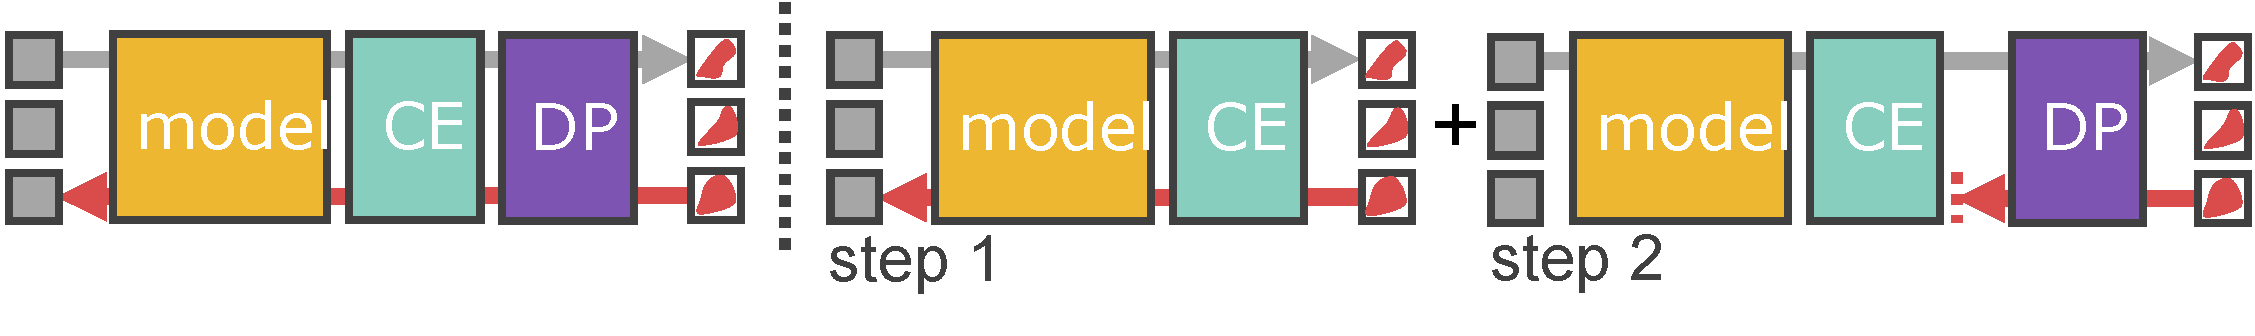
\includegraphics[width=\textwidth]{\deepstaplePath/figures/dp_backprop_twostep}
            \caption{\textbf{Left:} Inline backpropagation updating (red arrow) model and data parameters together. \textbf{Right:} Out-of-line backpropagation first steps on model (gray arrow) using normal cross-entropy loss and then steps on data parameters using the model's weights of the first step.}
            \label{fig:ool_backprop}
        \end{figure}
        First only the main model parameters will be optimized. Secondly only the data parameters will be optimized \emph{out-of-line}.
        % leaving the main model parameters untouched.
        % We suppose that in training scenarios with severe noise when a generalized solution is harder to find the model learning process can be interfered by the inline data parameter optimization.
        When using the \emph{out-of-line}, two-step approach data parameter optimization becomes a hypothesis of \emph{``what would help the model optimizing right now?''} without intervening. Due to the optimizer momentum the parameter values still become reasonably separated.
        % This in term will not directly increase the model scores in training but the learned data parameters can be applied in a second run as a fixed pre-weighting or be extracted for further usage (see next paragaraph).

    \paragraph{\textbf{Consensus generation via weighted voting}}
        \label{sec:consensus}
        % For weighting of label atlases and fusion numerous techniques exist like majority voting \citep{rohlfing2004performance} or STAPLE \citep{warfield2004simultaneous}.
        To create a consensus \(\mathbf{C_M}\) we use a simple weighted-sum over a set of multi-atlas labels \(M\) associated to a fixed image that turned out to be effective
        \begin{equation}
            \label{eq:weighted_sum}
            \mathbf{C_M} = \left(\sum_{m=1}^{\lvert M \rvert} softmax(\mathbf{DP_{M}})_{m} \cdot \mathbf{y_m}\right) > 0.5 \quad \textrm{with} \quad M \subset S
        \end{equation}
        where \(\mathbf{DP_{M}}\) are the parameters associated to the set of multi-atlas labels \(\mathbf{y_M}\).


\newpage
\section{Experiments and Results}
    \label{sec:experiments_deepstaple}
    In this section, we will describe general dataset and model properties as well as our four experiments which increase in complexity up to the successful application of our method in 3D multi-atlas label noise estimation. We will refer to oracle-labels\footnote{``The word oracle [...] properly refers to the priest or priestess uttering the prediction.''. ``Oracle.'' Wikipedia, Wikimedia Foundation, 03 Feb 2022, en.wikipedia.org/wiki/Oracle} as the real target labels which belong to an image and “registered/training/ground-truth”-labels as image labels that the network used to update its weights. Oracle-Dice refers to the overlapping area of oracle-labels and “registered/training/ground-truth”-labels.
    % The experiments are structured as follows:
    % 2D model training with artificially disturbed (experiment I), 2D model training with a quality-mix of registered single-atlas labels (experiment II), 3D registered  multi-atlas labels (experiment III) and consensus generation and subsequent network training (experiment IV).
    % \begin{itemize}[wide=0pt, leftmargin=\parindent, widest=99]
    % \begin{itemize}[wide=0pt,labelwidth=4em,leftmargin=\parindent, widest=99]
    %     \item[EXP I] 2D model training, artificially disturbed ground-truth labels
    %     \item[EXP II] 2D model training, quality-mixed registered single-atlas labels
    %     \item[EXP III] 3D model training, registered multi-atlas labels
    %     \item[EXP IV] Consensus generation and subsequent network training \label{last-item}
    % \end{itemize}

    % \vspace{-7pt}
    \paragraph{\textbf{Dataset}}
    For our experiments, we chose a challenging multimodal segmentation task which was part of the CrossMoDa challenge \citep{shapey2021segmentation}. The data contains contrast-enhanced T1-weighted brain tumour MRI scans and high-resolution T2-weighted images (initial resolution of \(384/448\times348/448\times80~vox\) @ \(0.5~mm\times0.5~mm\times1.0-1.5~mm\) and \(512\times512\times120~vox\) @ \(0.4\times0.4\times1.0 - 1.5~mm\)).
    We used the original TCIA dataset \citep{shapey2021segmentation} to provide omitted labels of the CrossModa challenge which served as oracle-labels.
    Prior to training isotropic resampling to \(0.5~mm\times0.5~mm\times0.5~mm\) was performed as well as cropping the data to \(128\times128\times128~vox\) around the tumour. We omitted the provided cochlea labels and train on binary masks of background/tumour. As the tumour is either contained on the right- or left side of the hemisphere, we flipped the right samples to provide pre-oriented training data and omit the data without tumour structures. For the 2D experiments we sliced the last data dimension.
    % \footnote{Preprocessing scripts can be found in our code repository on GitHub}.

    % \vspace{-7pt}
    \paragraph{\textbf{Model and training settings}}
    % As our main model we use a 2D-MobileNetV3 \citep{howard2019searching} and a custom 3D-MobileNet backbone similar to MobileNetV2 \citep{sandler2018mobilenetv2} with aspp pooling and an LR-ASPP head \citep{howard2019searching}.
    For 2D segmentation, we employ a LR-ASPP MobileNetV3-Large model \citep{howard2019searching}. For 3D experiments we use a custom 3D-MobileNet backbone similar as proposed in \citep{sandler2018mobilenetv2} with an adapted 3D-LR-ASPP head \citep{hempe2022opportunistic}.
    % The custom 3D-MobileNet backbone consists of 10 depth-separable convolution blocks with inverted residual connections at block 2,4,9 and 10. The resolution is reduced with stride 2 in block 1 and 7. The resulting backbone holds 223k trainable parameters.
    2D training was performed with an AdamW \citep{loshchilov2017decoupled} optimizer with a learning rate of \(\lambda_{2D}=0.0005\),
    \(\lvert B \rvert_{2D}=32\), cosine annealing \citep{loshchilov2016sgdr} as scheduling method with restart after \(t_0=500\) batch steps and multiplication factor of 2.0.
    For the data parameters, we used the SparseAdam-optimizer implementation together with the sparse Embedding structure of PyTorch with a learning rate of \(\lambda_{DP}=0.1\), no scheduling, \(\beta_1=0.9\) and \(\beta_2=0.999\).
    % the same first and second order momentum as AdamW.
    % As \citep{Castells.2020} stated, this additional optimizer also introduces additional hyperparameters, but we just followed \citep{saxena2019data} and set the learning rate to the suggested value without further adjustments.
    3D training was conducted with learning rate of \(\lambda_{3D}=0.01\), \(\lvert B \rvert_{3D}=8\) due to memory restrictions and exponentially decayed scheduling with factor of \(d=0.99\). As opposed to Saxena et al. \citep{saxena2019data} during our experiments we did not find weight-clipping, weight decay or \(\ell_{2}\)-regularisation on data parameters to be necessary. Parameters \(DP_s\) were initialized with a value of 0.0.
    For all experiments, we used spatial affine- and b-spline-augmentation and random-noise-augmentation on image intensities.
    Prior to augmenting we upscaled the input images and labels to \(256\times256~px\) in 2D- and \(192\times192\times192~vox\) in 3D-training.
    % in 3D training which increased performance of the LRASPP variants significantly.
    Data was split into \(2/3\) training and \(1/3\) validation images during all runs and used global class weights \(1/{n_{bins}}^{0.35}\). %TODO edit bincount formula
    % \paragraph{\textbf{Metrics}}
    % \label{sec:metrics}
    % During our experiments we used the 2D- and 3D-DICE metric to evaluate prediction quality of the model as well as the consensus quality. We also measured the pearson correlation coefficient between the values of the training data parameters and the oracle dice i.e. the dice score between the provided training-label and the expert/“true” label which was not shown to the network during training.
    % \paragraph{\textbf{Baselines}}
    % \label{sec:baselines}

    % For experiment I-III we benchmark our results against the same model without data parameters and standard cross-entropy loss. For experiment IV we use randomly selected registered labels as lower and oracle-labels as upper baseline. We refer to the Dice score between a label and the oracle-label as the ``oracle dice''.

    \begin{figure}
        \definecolor{amethyst}{rgb}{0.60,0.40,0.80}
        \definecolor{amber}{rgb}{1.00,0.75,0.00}
        \definecolor{applegreen}{rgb}{0.55,0.71,0.00}
        \definecolor{amber(sae/ece)}{rgb}{1.00,0.49,0.00}
        \centering
        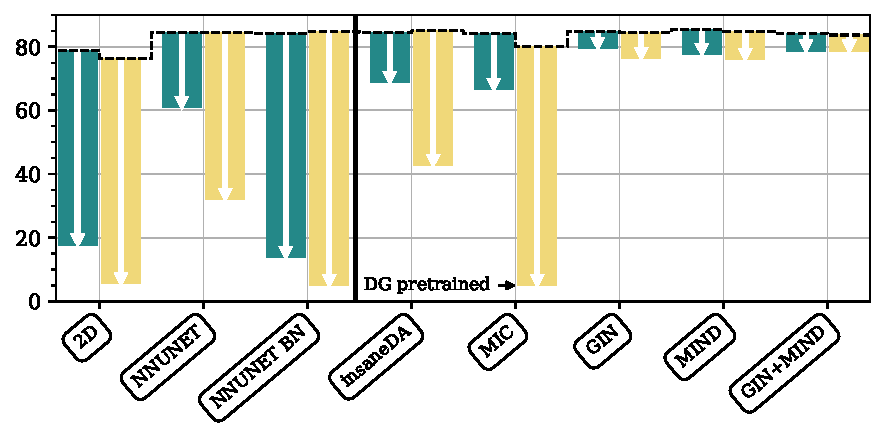
\includegraphics[width=\textwidth]{\deepstaplePath/figures/exp1}
        \caption{\textbf{Left:} Sample disturbance \legendbox{red} at strengths [0.1, 0.5, 1.0, 5.0]. \textbf{Middle:} Validation Dice when training with named disturbance strenghts, either with data parameters enabled (\sampleline{}) or disabled (\sampleline{dashed}). \textbf{Right:} Parameter distribution for combinations of risk regularization (RR) and fixed weighting (FW): RR+FW \legendbox{amethyst} |~RR \legendbox{amber(sae/ece)} |~FW \legendbox{amber}  |~NONE \legendbox{applegreen}. Saturated data points indicate higher oracle-Dice. Value of ranked Spearman-correlation \(r_s\) between data parameters and oracle-Dice given.}
        \label{fig:exp1_deepstaple}
        % \vspace{-12pt}
    \end{figure}
    % \vspace{-7pt}

    \paragraph{\textbf{Experiment I: 2D model training, artificially disturbed ground-truth labels}}
    This experiment shows the general applicability of data parameters in the semantic segmentation setting when using one parameter per 2D slice.
    % when training on labels in the T1-weighted image domain.
    To simulate label-noise, we shifted 30\% of the non-empty oracle-slices with different strengths (Fig. \ref{fig:exp1_deepstaple}, left) to see how the network scores behave (Fig. \ref{fig:exp1_deepstaple}, middle) and whether the data parameter distribution captures the artificially disturbed samples (Fig. \ref{fig:exp1_deepstaple}, right).
    % for runs with and without data parameters enabled.
    In case of runs with data parameters the optimization was enabled after 10 epochs.
    % colored by oracle dice of a selected run of 1.0 disturbance strength.
    % \vspace{-7pt}

    \paragraph{\textbf{Experiment II: 2D model training, quality-mixed registered single-atlas labels}}
    Extending experiment I, in this setting we train on real registration noise with 2D slices on single-atlases.
    We use 30 T1-weighted images as fixed targets (non-labelled) and T2-weighted images and labels as moving pairs. For registration we use the deep learning-based algorithm Convex Adam \citep{siebert2021fast}. We select two registration qualities to show quality influence during training: \emph{Best}-quality registration means the single best registration with an average of around 80\% oracle-Dice across all atlas registrations. \emph{Combined}-quality means a clipped, gaussian-blurred sum of all 30 registered atlas registrations (some sort of consensus).
    We then input a mix of 50\%/50\% randomly selected best/combined labels into training. Afterwards we compare the 100\% best, 50\%/50\% mixed and 100\% combined selections focusing on the mixed setting where we train with and without data parameters. Validation scores were as follows (descending): best@no-data-parameters 81.1\%, mix@data-parameters 74.1\%, mix@no-data-parameters 69.6\% and combined@no-data-parameters 61.9\%.

    \begin{figure}
        \centering
        \begin{minipage}[b]{0.31\textwidth}
            \centering
            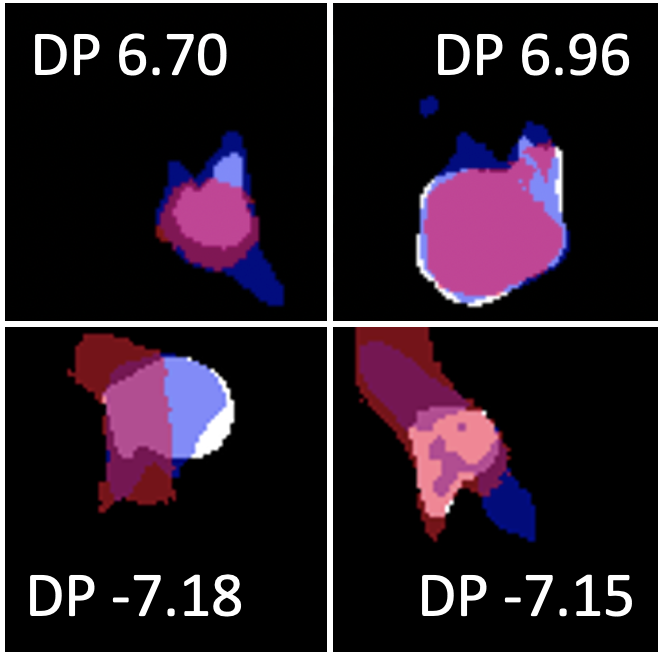
\includegraphics[width=.9\textwidth]{\deepstaplePath/figures/exp2_dp_vals.png}
        \end{minipage}
        \hfill
        \begin{minipage}[b]{0.31\textwidth}
            \centering
            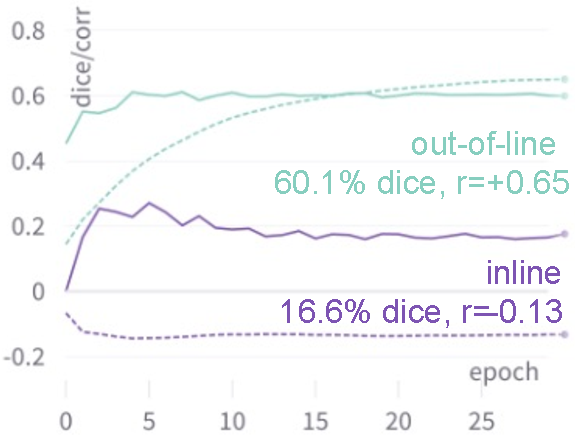
\includegraphics[width=\textwidth]{\deepstaplePath/figures/exp3_scores_drop}
        \end{minipage}
        \hfill
        \begin{minipage}[b]{0.33\textwidth}
            \centering
            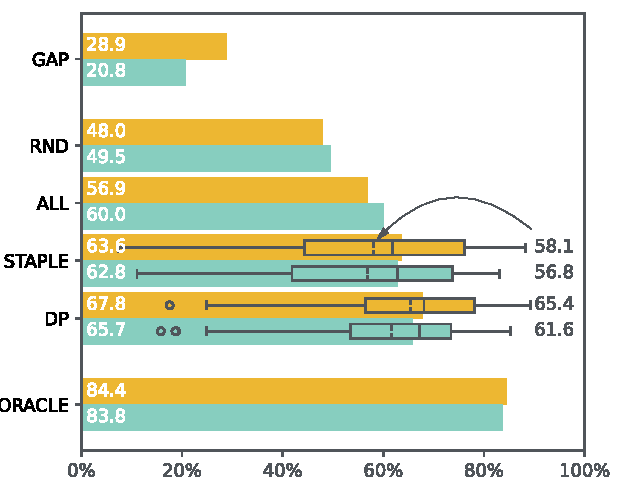
\includegraphics[width=\textwidth]{\deepstaplePath/figures/exp4_boxplot_enhanced}
        \end{minipage}
        \par
        \begin{minipage}{0.31\linewidth}
            \caption{Selected samples with low- and high parameters: Oracle-label \legendboxoutline{white}, network prediction \legendbox{regblue} and deeds registered label \legendbox{regred}} \label{fig:epx2_dp_vals}
        \end{minipage}
        \hfill
        \begin{minipage}{0.31\linewidth}
            \caption{%
                Inline \legendbox{purple} and out-of-line \legendbox{green} backpropagation. Validation Dice (\sampleline{}) and Spearman-corr. of params. and oracle-Dice (\sampleline{dashed})%
            } \label{fig:exp3_scores_drop}
        \end{minipage}
        \hfill
        \begin{minipage}{0.33\linewidth}
            % \caption{\textbf{FG:} Boxplots showing STAPLE \legendbox{red} and DP \legendbox{green} consensus (median \sampleline{}, mean \sampleline{dashed}). \textbf{BG:} nnUNet training scores \legendbox{yellow} with: randomly selected atlases, consensi and oracle-labels}
            \caption{\textbf{FG:} Box plots of STAPLE and DP consensus quality, mean value on the right. \textbf{BG:} Bar plot of nnUNet scores; deeds \legendbox{green}, Convex Adam \legendbox{yellow}}
            \label{fig:exp4_boxplot}
        \end{minipage}
        % \vspace{-12pt}
    \end{figure}

    % \vspace{-7pt}
    \paragraph{\textbf{Experiment III: 3D model training, registered multi-atlas labels}}
    Extending experiment II, in this setting we train on real registration noise but with 3D volumes and multiple atlases per image.
    We follow the CrossMoDa \citep{shapey2021segmentation} challenge task and use T2-weighted images as fixed targets (non-labelled) and T1-weighted images and labels as moving pairs. We conducted registration with two algorithms (iterative deeds \citep{heinrich2012globally} and deep learning-based algorithm Convex Adam \citep{siebert2021fast}). For each registration method 10 registered atlases per image are fed to the training routine expanding the T2-weighted training size from 40 to 400 label-image pairs each.
    Fig. \ref{fig:exp3_scores_drop} shows a run with inline and out-of-line (see Sec. \ref{sec:ool_backprop}) data parameter training on the deeds registrations as an example how training scores behave.

    % \vspace{-7pt}
    \paragraph{\textbf{Experiment IV: Consensus generation and subsequent network training}}
    Using the training output of experiment III, we built 2x40 consensi: [10 deeds registered @ 40 fixed] and [10 Convex Adam registered @ 40 fixed]. Consensi were built by applying the STAPLE algorithm as baseline and opposed to that our proposed weighted-sum method on data parameters (DP) (see Sec. \ref{sec:fixed_weighting}).
    On these, we trained several powerful nnUnet-models for segmentation
    % --- more powerful but also more resource demanding segmentation models which employ various techniques in pre- and postprocessing to optimize segmentation results
    \citep{isensee2021nnu}.
    % Fig. \ref{fig:exp4_boxplot} shows the oracle-Dice distribution of 40 consensi (10 registered @ 40 fixed T2 images) as well as the mean validation Dice of a subsequent nnUnet-model training \citep{isensee2021nnu} after 150 training epochs for 40 randomly selected atlas labels (RND, 48.0\%), 40 STAPLE consensi (63.6\%), 40 data parameter consensi (DP, 67.8\%) and 40 oracle-labels (84.4\%).
    In Fig. \ref{fig:exp4_boxplot} in the foreground four box plots show the quality range of generated consensi regarding the oracle dice: [deeds, Convex Adam registrations]@[STAPLE, DP].
    In the background the mean validation Dice of nnUnet-model trainings (150 epochs) is shown. As a reference, we trained directly on the T1-moving data with strong data augmentation (nnUNet ``insane'' augmentation) trying to overcome the domain gap directly (GAP). Furthermore, we trained on 40 randomly selected atlas labels (RND), all 400 atlas labels (ALL), STAPLE consensi, data parameter consensi (DP) and oracle-labels either on deeds or Convex Adam registered data. Note that the deeds data contained 40 unique moving atlases whereas the Convex Adam data contained 20 unique moving atlases, both warped to 40 fixed images as stated before.
    % Pay attention to boxplots STAPLE vs. DP (ours) and foreground vs. background i.e. consensus mean and subsequent nnUNet mean validation score when trained on the corresponding consensus.

    \label{sec:results}
    In \textbf{experiment I} we could show that our usage of data parameters is generally effective in the semantic segmentation scenario under artificial label noise.
    Fig. \ref{fig:exp1_deepstaple} (middle) shows an increase of validation scores when activating stepping on data parameters after 10 epochs for disturbance strengths \(>0.1\). Stronger disturbances lead to more severe score drops but can be recovered by using data parameters.
    In Fig. \ref{fig:exp1_deepstaple} (right) one can see that data parameters and oracle-Dice correlate most, when using the proposed risk regularization as well as the fixed weighting-scheme configuration (see Sec. \ref{sec:method_deepstaple}). We did not notice any validation score improvements when switching between configurations and therefore conclude that a sorting of samples can also be learned inherently by the network. However, properly weighted data parameters can extract this information, make it explicitly visible and increase explainability.
    In \textbf{experiment II} we show that our approach works for registration noise during 2D training: When comparing different registration qualities, we observed that training scores drop from 81.1\% to 69.6\% Dice when lowering registration input quality. By using data parameters we can recover to a score of 74.1\% meaning an improvement of +4.5\%.
    \textbf{Experiment III} covers our target scenario --- 3D training with registered multi-atlas labels. With inline training of data parameters (used in the former experiments), validation scores during training drop significantly. Furthermore the data parameters do not separate high- and low quality registered atlases well (see Fig. \ref{fig:exp3_scores_drop}, inline). When using our proposed out-of-line training approach (see Sec. \ref{sec:ool_backprop}) validation Dice and ranked correlation of data parameter values and oracle-Dice improve.
    \textbf{Experiment IV} shows that data parameters can be used to create a weighted-sum consensus as described in Sec. \ref{sec:fixed_weighting}: Using data parameters, we can improve mean consensus-Dice for both, deeds and Convex Adam registrations over STAPLE \citep{warfield2004simultaneous} from 58.1\% to 64.3\% (+6.2\%, ours, deeds data) and 56.8\% to 61.6\% (+4.8\%, ours, Convex Adam data).
    When using the consensi in a subsequent nnUNet training \citep{isensee2021nnu}, scores behave likewise (see Fig. \ref{fig:exp4_boxplot}).
      % We suppose the fixed weighting to be related to the cross-entropy mean reduction which should not be inherited into the data parameters values because it is of no use classifying spatially larger propagated labels to be more noisy than smaller labels in general.
    % This seems reasonable since the STAPLE algorithm only takes registered labels as inputs and has no information about the image intensity context our network training captures during training.
    Regarding training times of over an hour with our LR-ASPP MobileNetV3-Large training, one has to consider that applying the STAPLE algorithm is magnitudes faster.
    % However network training yields the opportunity to furthermore predict segmentations on the target domain directly.
    % Additionally, sorting all training samples by their data parameter value can give researchers a valuable insight into the dataset sample quality distribution in general to optimize network training data prior to experimenting with new methods. TODO probably move this.
    % TODO: Add other CrossMoDa results
% \begin{figure}
%     \centering
%     \begin{minipage}[b]{0.45\linewidth}
%         \centering
%         \expfourimg
%         \caption{Histogram of consensi when compared to the expert label}
%         \label{fig:exp4_consensus}
%     \end{minipage}
%     \hfill
%     \begin{minipage}[b]{0.45\linewidth}
%         \centering
%         \expfourtab
%         \captionof{table}{nnUNet training mean dices for declared sub-experiments}
%         \label{tab:exp4_nnunet}
%     \end{minipage}
% \end{figure}

\section{Discussion and Conclusion}
    \label{sec:conclusion}
    Within this work, we showed that using data parameters in a multimodal prediction setting with propagated source labels is a valid approach to improve network training scores, get insight into training data quality and use the extracted info about sample quality in subsequent steps namely to generate consensus segmentations and provide these to further steps of deep learning pipelines. Our improvements over the original data parameter approach for semantic segmentation show strong results in both 2D- and 3D-training settings. Although we could extract sample quality information in the multi-atlas setting successfully, we could not improve network training scores in this setting directly since using the data parameters inline of the training loop resulted in unstable training.
    Regarding that, we want to continue investigating how an inline training can directly improve training scores in the multi-atlas setting. Furthermore our empirically chosen fixed weighting needs more theoretical foundation. The consensus generation could be further improved by trying more complex weighting schemes or incorporating the network predictions itself. Also we would like to compare our registration-segmentation pipeline against specialized approaches of Ding et al. and Liu et al. \citep{ding2019votenet,ding2020votenet+,liu2021style} which we consider as very interesting baselines.
